% Copy this folder, replace metadata/body/bibliography, then compile with latexmk -xelatex.
\documentclass[UTF8,a4paper,fontset=fandol,zihao=5,openany]{ctexrep}
\usepackage[margin=25.4mm]{geometry}
\usepackage{graphicx,booktabs,amsmath}
\usepackage[sort&compress]{gbt7714}
\usepackage{caption}
\usepackage[hidelinks]{hyperref}
\IfFontExistsTF{Times New Roman}{\setmainfont{Times New Roman}}{\setmainfont{TeX Gyre Termes}}
% Fandol is bundled with TeX Live: deterministic CJK choice on Windows and macOS.
\ctexset{
  chapter={format=\centering\heiti\bfseries\fontsize{16}{20}\selectfont,
    beforeskip=12pt,afterskip=6pt},
  section={format=\heiti\bfseries\fontsize{14}{18}\selectfont},
  subsection={format=\heiti\bfseries\fontsize{12}{16}\selectfont}}
\setlength{\parindent}{2em}
\setlength{\parskip}{6pt}
\captionsetup{position=bottom,font=small,labelsep=space}
\renewcommand{\bibfont}{\fontsize{10}{12}\selectfont}
\setcounter{tocdepth}{2}


\usepackage{float}
\hypersetup{pdftitle={大语言模型驱动的多智能体协作研究综述},pdfauthor={技术综述产出测试}}
\begin{document}
\fontsize{10.5}{13.125}\selectfont
\pagestyle{empty}
\begin{titlepage}
\centering
\vspace*{28mm}
{\heiti\bfseries\fontsize{22}{30}\selectfont 技术综述产出测试\par}
\vspace{24mm}
{\heiti\bfseries\fontsize{20}{30}\selectfont 大语言模型驱动的\par 多智能体协作研究综述\par}
\vspace{22mm}
{\fontsize{13}{24}\selectfont 从组织机制到可验证的协作收益\par}
\vspace{15mm}
{\fontsize{11}{20}\selectfont 文献范围：经典基础与2023—2026年代表性工作\par 检索截止：2026年10月27日\par}
\vfill
{2026年10月27日\par}
\vspace*{15mm}
\end{titlepage}
\pagenumbering{gobble}
\tableofcontents
\thispagestyle{empty}
\clearpage
\pagenumbering{arabic}
\pagestyle{plain}

\chapter{引言}

\section{问题背景与研究范围}
多智能体研究关注多个具有一定自主性的决策主体如何在共享或相互影响的环境中行动。经典智能体理论把自主性、反应性、主动性与社会交互能力视为理解智能体的重要线索，不能仅以程序数量或对话窗口数量判定系统是否具备有效协作能力。\cite{wooldridge} 本文所说的“大语言模型驱动多智能体”，主要指以语言模型承担部分推理与决策功能、通过消息和工具共同推进任务的系统。不同智能体可以使用同一基础模型，但拥有不同上下文、工具权限和职责。

这一方向受到关注，是因为复杂任务常包含知识检索、方案生成、程序执行与结果核验等异质环节。将任务分配给多个主体，理论上可扩大信息覆盖、并行处理可分解工作，并为错误提供交叉检查机会。然而，分工同时引入信息交接、状态同步、冲突裁决与停止判定成本。报告的中心问题因此是：在什么任务和资源约束下，协作带来的互补收益能够超过这些成本？“增加智能体”本身不是充分答案。

本文以大语言模型协作为重点，并区分三条相互关联但不能混同的研究路线：经典多智能体系统研究自主主体之间的组织与交互；多智能体强化学习研究交互环境中的策略学习；大语言模型多智能体研究则大量采用提示、工具调用与工作流编排，也可以进一步引入协作训练。它们共享协调、局部信息与信用分配等问题，使用的表示、学习方式和评价对象并不相同。


\section{资料范围与证据边界}
本文于2026年10月27日完成选择性检索，覆盖经典智能体与强化学习基础、2023—2025年代表性语言模型协作框架和训练方法，以及2026年可核验的系统比较、部分可观测协作、长程任务评测和伙伴探索研究。主要查阅arXiv版本化论文、ACL与PMLR等官方论文集、期刊出版页面及论文全文。该范围用于建立有代表性的分析框架，不构成穷尽式系统综述，也不以论文数量推断热点的流行程度。

报告区分文献报告的事实、根据这些事实作出的分析和建议开展的研究。文中基准结果均来自原论文，未开展新的模型训练或性能复现实验。框架可以实现某种流程，不等于该流程在任意任务上优于强单智能体；模拟社会中的可信行为，也不等于对真实社会规律的验证。后文“个人思考”是报告作者的分析判断，不代表亲历实验或用户个人经历。


\chapter{已有工作概述}

\section{从交互决策到可学习的协作}
经典多智能体思想强调主体之间的知识、目标和行动关系。进入深度强化学习阶段，一个突出问题是：其他智能体的策略也在变化，使单个主体看到的环境具有非平稳性。MADDPG把其他智能体的信息纳入训练阶段的评价机制，在合作与竞争环境中学习协调策略；其价值在于说明训练时利用联合信息与执行时保持局部决策可以相结合。\cite{maddpg}

QMIX进一步以联合行动价值的单调分解实现集中训练与分散执行，在特定结构约束下保证局部贪心动作与联合价值最大化的一致性，并在星际争霸微操任务中评价。\cite{qmix} 这里的“集中训练”不是由一个语言模型担任组长，“分散执行”也不是简单开启多个聊天机器人。前者涉及策略参数、价值估计和环境奖励，后者首先是推理时的信息与控制组织。区分这两层，才能判断一个工作到底改变了模型能力，还是只改变了调用方式。

语言模型智能体的一个基础是把推理与环境行动连接起来。ReAct将推理轨迹与任务动作交错组织，使模型通过外部反馈更新行动计划。\cite{react} 它主要提供单智能体的行动循环，不能直接作为多智能体优越性的证据；但它说明，多智能体团队中的每个成员也需要可靠的观察、行动与反馈链条，单纯交换意见不足以完成开放环境中的任务。


\section{对话框架、角色分工与记忆机制}
AutoGen把可对话智能体作为通用接口，允许语言模型、工具和人类输入以不同组合参与可编程交互。其重要贡献是降低多主体流程的实现门槛，开发者可以设计轮流对话、层级协作或按条件调用的模式。\cite{autogen} 这种灵活性同时意味着，实际效果高度依赖任务分解、工具权限和终止规则。框架提供能力接口，并不替代系统设计和公平评测。

MetaGPT把标准操作流程引入多智能体软件开发，利用产品、设计、编码等角色组织中间产物与交接顺序。\cite{metagpt} 相比无约束群聊，明确产物格式与依赖关系有助于减少协作歧义。其思想可以推广为：每个角色都应有具体输入、输出和可检查责任，而不是只有一个职业名称。本文不把论文中的特定软件任务结果扩展为所有领域的普适优势。

另一条路线是生成式社会模拟。Generative Agents通过记忆、反思与规划，在包含25个智能体的小镇环境中产生具有可信性的行为与社交互动。\cite{generative} 其评价重点包括行为可信度，目标与求解任务的正确率不同。记忆架构具有启发性，但“像人”与“正确完成团队任务”是两个评价维度；拟人化角色并不能自然保证工程可靠性。

图2.1概括本文对任务型协作的综合理解：任务约束决定分解与预算路由，专业成员在证据与共享状态的支持下工作，集成结果还需要外部验证；失败反馈触发有限返工或人工升级。该图是文献综合形成的概念架构，不是所有框架的统一实现，也不表示已经测得任何性能提升。


\begin{figure}[H]
\centering
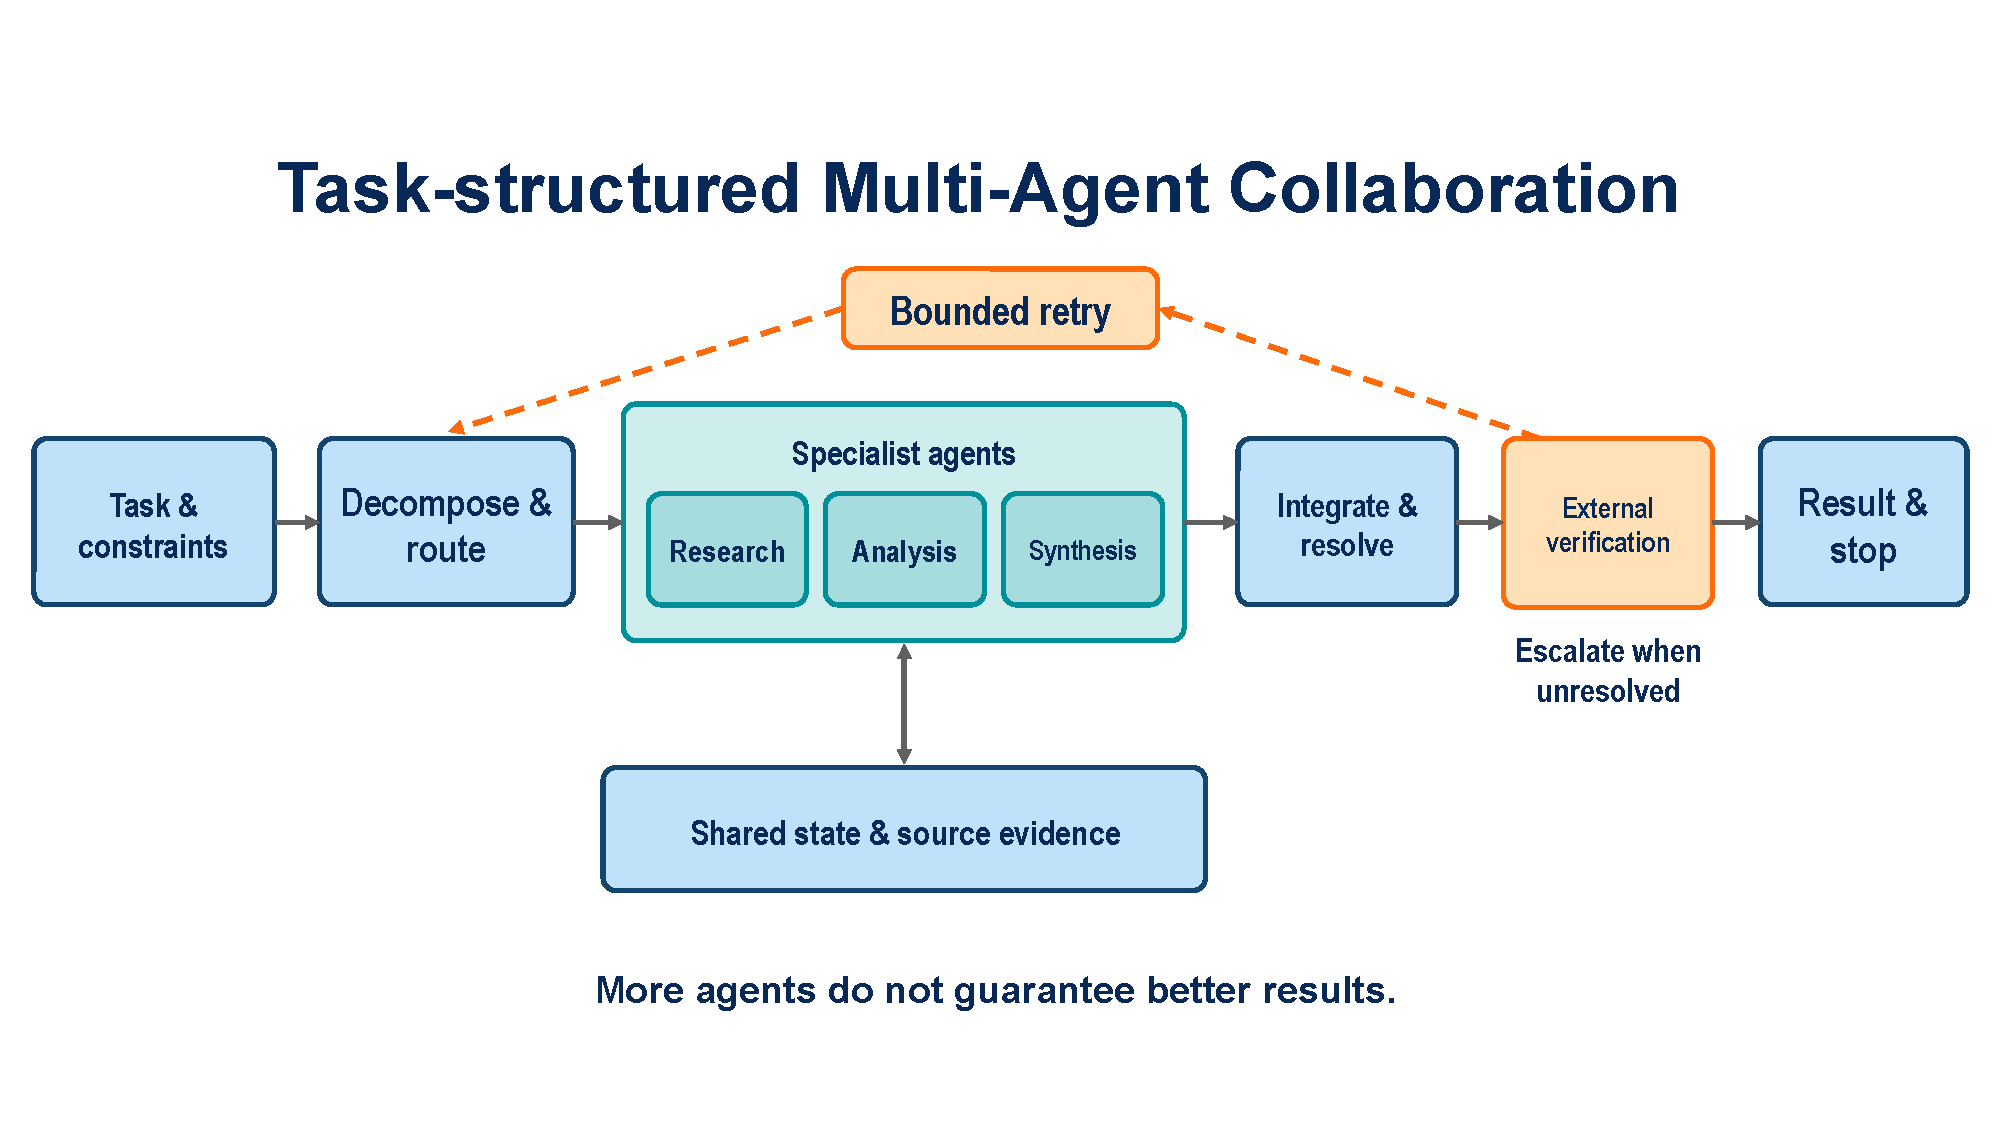
\includegraphics[width=.96\linewidth]{assets/collaboration-figure.pdf}
\caption{概念图：任务结构驱动的多智能体协作}\label{fig:collaboration}
\end{figure}

\section{从框架展示走向过程评测与协作训练}
MultiAgentBench把协作与竞争放到多个交互场景中评价，除任务完成外，还关注基于里程碑的过程指标，并比较不同协调拓扑。\cite{multiagentbench} 这类工作的重要性是把评价单位从“最后回答是否正确”扩展到“团队如何取得进展”。但不同场景对通信的需求不同，在研究场景中表现较好的拓扑，不应被直接认定为所有任务的最优结构。

MAST从实际执行轨迹出发，总结系统设计、智能体间失配与任务验证三类问题，共14种细粒度失败模式。\cite{mast} 它揭示了一种常见现象：团队可能重复步骤、丢失上下文，或在没有完成有效核验时宣布成功。该研究主要提供失败分类与诊断依据，不能把不同任务上的框架失败分布直接排列成统一性能榜，也不能由分类频率自动推导因果机制。

MAPoRL则把协作从推理时的提示设计推进到联合后训练：模型先独立生成，再讨论，利用验证器提供的奖励及纠错、说服激励进行多智能体强化学习。\cite{maporl} 这表明协作行为可以成为训练目标，冻结模型的多轮讨论并不是唯一技术路线。但训练后的增益仍需结合训练数据、奖励设计和测试领域理解，不能仅凭加入强化学习便断言具备通用合作能力。


\chapter{当前热点研究方向}

\section{面向任务结构的编排与成本控制}
近年活跃的一个问题是如何选择智能体数量、通信拓扑与工作流，而2026年的受控比较进一步凸显了强单智能体基线的重要性。Kim等在六类任务、五种架构和三个模型家族的260种配置上控制提示、工具与计算预算，发现协作收益具有明显的任务依赖性。论文将能力饱和阈值解释为实际选型规则，而不是普适尺度定律；其跨域绝对预测能力也受到限制。\cite{scaling}

由此可作出的分析是，编排应首先判断依赖结构。独立资料搜集、候选方案探索等工作有较多并行空间；严格依赖前一步状态的操作，频繁交接则可能破坏连续性。静态多角色流程适用于依赖明确、重复执行的任务，动态路由适用于能力和信息分布变化较大的任务。动态系统也必须支付路由决策成本，因此“更灵活”不能直接等同于“更高效”。

评价成本时，应同时记录输入输出token、工具调用、墙钟时延与失败后的返工。只比较总调用次数会忽略每次上下文长度，只比较通信字数又会漏掉生成路由决策的成本。合理的研究问题不是哪个架构单点分数最高，而是在给定预算下，哪些架构位于质量、时间与费用的有效权衡边界上。


\section{部分可观测条件下的通信、记忆与伙伴选择}
真实协作常存在知识与权限边界：某个成员拥有局部文件，另一个成员掌握执行工具，团队需要交换必要信息，而非复制所有上下文。2026年10月的MASBench围绕推理、调度与游戏三类任务，分别考察协议、记忆和路由机制，并设置确定性的任务评价。值得注意的是，其主要通信成本指标不包括各智能体的本地推理token，附录还区分了传输消息成本与完整消息阶段生成成本。\cite{masbench}

这一边界对解释“效率提升”很关键：通信更短可能只是压缩了传输文本，系统总开销未必下降。共享记忆也应保留来源、时间和状态版本，防止过期判断被下游当作事实。上述设计要求属于本文的工程分析，而非对某一框架已实现能力的宣称。

伙伴选择是另一个已核实的新议题。2026年10月修订的研究把选择和探索协作者建模为部分可观测随机博弈，并用MACE引导探索；在所测问答与推理设置中，仅靠上下文中的历史信息可能导致过早偏向某个伙伴。\cite{exploration} 其结果支持显式探索机制的研究价值，但实验尚未建立数百、数千主体规模下的效果，理论保证也依赖明确假设。它不能证明任意开放智能体网络都适用同一种选择策略。


\section{长程协作、贡献归因与外部验证}
截至检索日，2026年9月发布的AgentWorld已把长程、非对称能力与资源共享纳入协作评测。其主任务集包含100个人工标注任务，在黑箱交互条件下，四个主要模型中最高任务成功率为52.0\%；这只是该基准与配置中的结果。论文还提出基于行动依赖图的因果协作有效性指标，以追踪哪些行动对结果产生贡献。\cite{agentworld}

这类指标有助于区分“团队很忙”与“团队有效”，但“因果”一词需要审慎理解：图上的贡献追踪不自动等同于严格干预实验中的因果效应，标注和评判机制本身也需要核验。成功率、部分完成度和过程贡献可以互补，不能互相替代。长程测试还应报告重跑方差与任务分布，避免把一次漂亮轨迹当成稳定能力。

可靠验证同样是近年持续活跃的问题。MAST中的验证类失败说明，安排一个审阅角色仍可能只得到表面检查。\cite{mast} 对代码应运行与需求有关的测试，对检索结论应回到原始资料，对操作型任务应读取环境最终状态。模型间一致意见可以作为线索，不能充当外部事实；程序可运行也不意味着业务要求已经满足。


\section{协作学习与评价目标的一致性}
联合后训练把“何时纠错、如何利用他人信息、何时停止讨论”转化为可学习行为，是MAPoRL等工作的研究方向。\cite{maporl} 其潜在优势是让模型在参数层面适应交互，但关键约束是奖励是否真正代表任务目标。若只奖励最终答案，关键的错误传播过程可能被掩盖；若过度奖励说服力，系统又可能优化表达而非正确性。

因此，训练目标宜同时检查结果质量、信息利用和成本约束，并用未见任务、未见伙伴或不同通信预算验证泛化。对冻结模型编排与协作训练的比较，应控制基础模型、训练数据和推理预算。否则，观察到的提升无法区分究竟来自更好的组织方式、额外训练，还是更高计算投入。


\chapter{未来研究}

\section{建立可检验的协作收益边界}
未来研究首先需要回答“什么时候值得协作”。可构建同时包含可并行子任务和严格顺序任务的评测集，预先定义分解粒度、信息重叠与状态依赖程度，再比较强单智能体、多次独立采样、固定工作流和动态团队。把多次采样纳入基线，是为了区分团队交互的收益与简单增加推理次数的收益。

实验应按任务来源或任务族划分训练与测试，避免模板近似的题目跨集合泄漏。统计单位应是独立任务或预先定义的重复运行，而不是把同一任务中的每条消息当作独立样本。本文建议报告任务配对差异、置信区间和成本分布；这些是实验设计建议，尚未实施，不能写成报告已经得到的结论。


\section{让共享状态和失败恢复成为研究对象}
长程协作需要可追踪的状态：哪些是直接观察，哪些是推断，谁在何时更新了它，哪些旧结论已失效。研究可比较全文共享、结构化共享和按需请求三种方式，测量状态一致性、有效信息保留率与总成本。评价信息压缩时，还要检查关键证据是否被删掉，不能仅以摘要更短判断更好。

失败恢复应区分暂时工具错误、证据不足和方案本身不可行。系统可以在预算内重试，但必须有停止与升级条件。检验恢复机制时，应在可控环境中注入缺失消息、过期状态或工具失败，并观察它是否发现问题、阻断传播以及保存可继续工作的成果。这样的干预更接近机制检验，比仅统计最终失败比例更能说明改动为何有效。


\section{学习面向陌生伙伴的可靠协作}
在开放团队中，伙伴能力、工具权限和反馈质量会变化。未来可将伙伴探索与任务路由联合研究：先用低成本任务估计伙伴可靠性，再随任务变化更新选择；同时限制探索成本，防止为了了解伙伴而消耗全部任务预算。验证重点应包括能力排序变化后的适应速度、低质量信息的扩散范围，以及合作与竞争目标发生冲突时的行为。

协作训练还应加入陌生伙伴测试，防止模型只学会适应固定队友的表达习惯。对于涉及外部系统的操作，需要将工具授权、执行记录和人工接管纳入系统边界。本文将这些视为未来评价与工程约束，不把它们描述成现有模型已经解决的问题。


\chapter{个人思考}

\section{先定义责任，再决定角色数量}
我的判断是，多智能体最有价值的设计单位是“可以验证的责任”，而不是拟人化头衔。检索成员应交付原始来源及支持位置，执行成员应交付日志与可检查结果，审阅成员应针对明确验收标准提出问题。如果一个角色只是复述其他成员的文字，它增加了调用链，却未必增加独立信息。

这也改变了我对“独立审查”的理解。角色名称不同不等于证据独立；若所有成员使用相同上下文与同一错误来源，团队仍可能一致犯错。更有意义的独立性来自不同的核验路径，例如用原始资料核查引用、用程序重算派生值、用环境状态检查操作完成。模型提供判断，外部证据承担事实约束。


\section{从最小闭环开始累积证据}
我倾向于先建立一个能完成任务且能检查结果的单智能体闭环，再仅对有明确并行空间或需要不同权限的部分增加成员。理由不是结构简单天然更强，而是较少的交接点使失败更容易定位，也能建立可信基线。若新增角色无法在相同资源预算下改善质量或时间，保留它便缺乏证据。

在研究报告和知识工作中，这意味着把作者、证据与审阅职责分清，并在有限修复轮次内完成可追踪交付。与其让多个模型反复给同一结论投票，我更重视每个关键判断能否指向原始材料，每次修改是否回应了已确认的缺陷。这是方法论立场，不是本文已经测得的性能优势。


\section{对未来能力保持可证伪的期待}
我认为该方向值得持续研究，尤其是部分可观测信息整合、长程状态管理和面向陌生伙伴的适应。不过，不能把协作视为基础模型能力不足时的通用补丁；强模型进步、预算变化与工具改进，都可能改变某种组织结构的价值。选择多智能体应由任务结构与比较证据共同支持。

本文的总体判断是：有效协作需要互补信息、明确责任、受控通信和外部验证共同成立。现有工作已经展示丰富实现路径，也揭示成本、失配与验证不足的边界。下一阶段更重要的进展，应体现在可重复的任务收益、可解释的失败减少与可衡量的资源效率上，而不是仅体现在团队规模或对话长度上。


\clearpage
\phantomsection
\addcontentsline{toc}{chapter}{参考文献}
\bibliographystyle{gbt7714-numerical}
\bibliography{references}
\end{document}
